\chapter{Grafische Auswertung der Untersuchungen}

\section{Untersuchung 35}

\begin{figure}[h!]
\centering
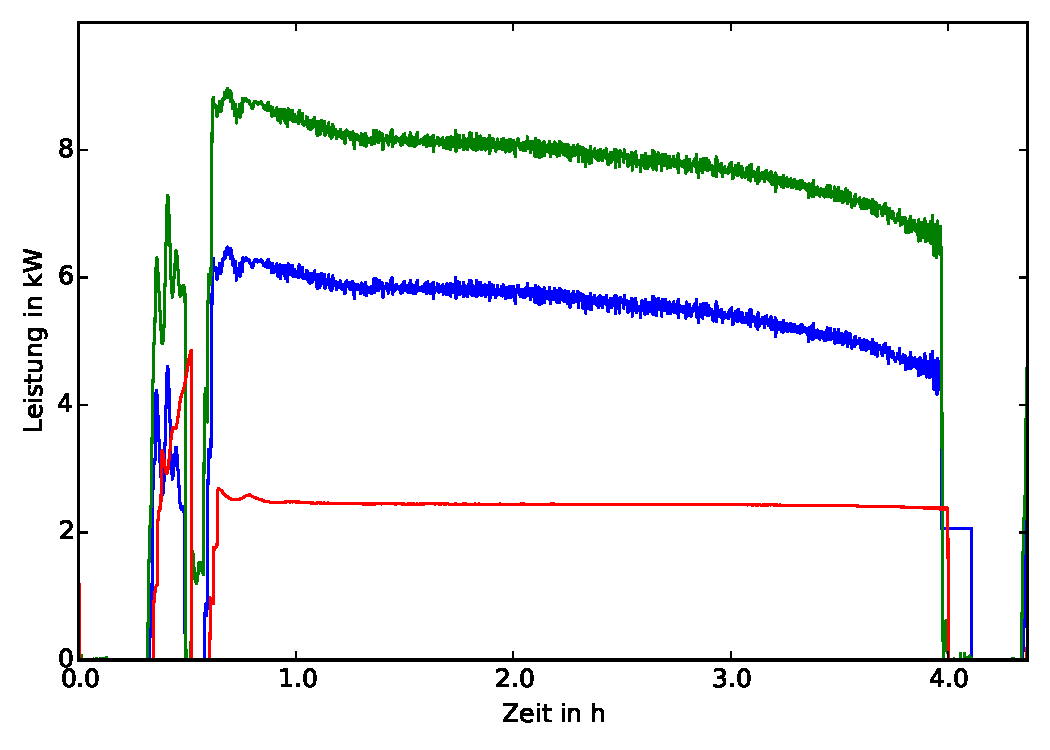
\includegraphics[scale=0.8]{Pictures/35/Qdots_lastCycle.pdf}
\caption{Leistungen beim Betrieb mit 3MAF.}
\label{fig:Leistungen35}
\end{figure}

\begin{figure}[h!]
\centering
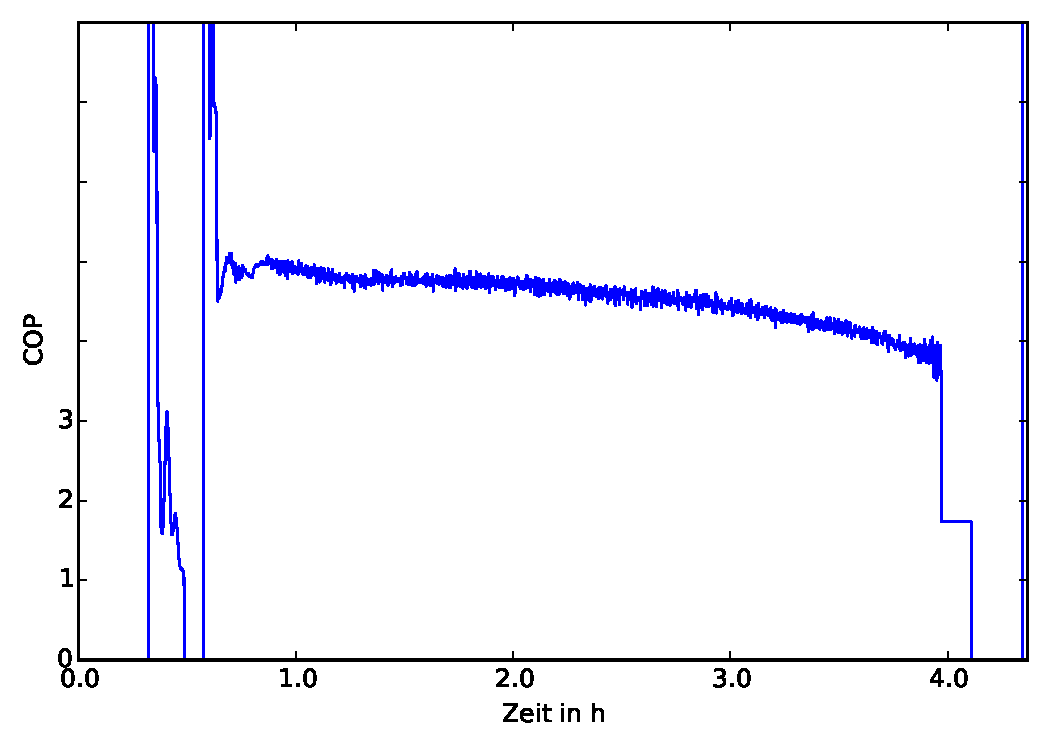
\includegraphics[scale=0.8]{Pictures/35/COP_lastCycle.pdf}
\caption{COP beim Betrieb mit 3MAF.}
\label{fig:COP35}
\end{figure}

\begin{figure}[h!]
\centering
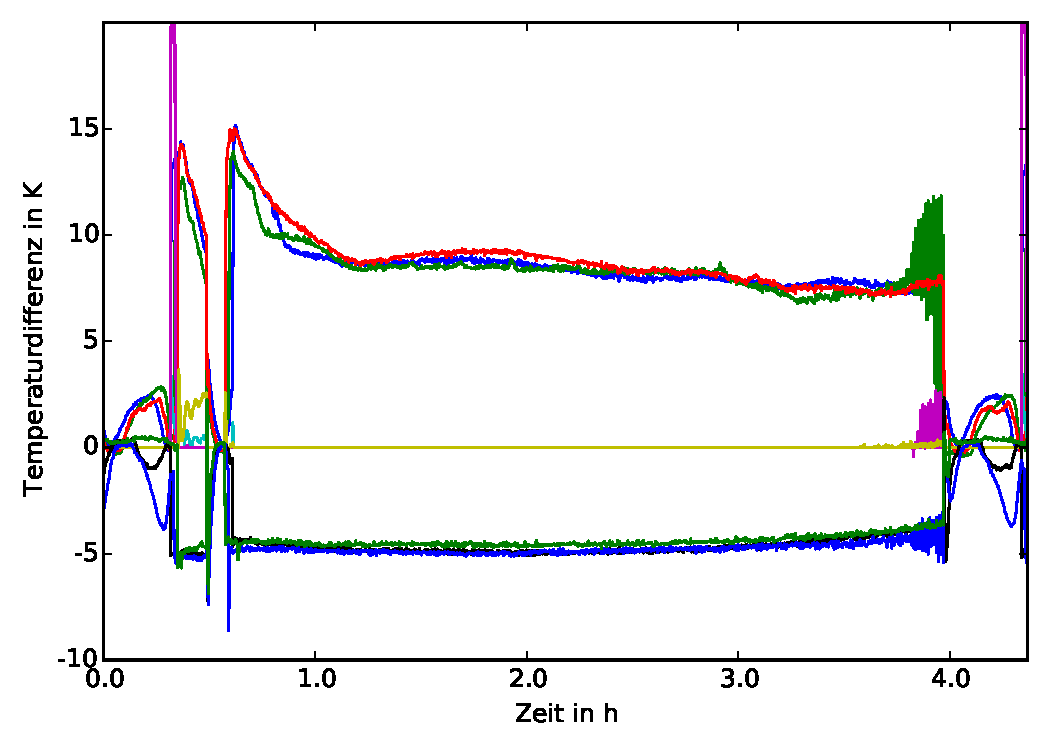
\includegraphics[scale=0.8]{Pictures/35/deltaTs_lastCycle.pdf}
\caption{Überhitzung und Unterkühlung (K1) beim Betrieb mit 3MAF.}
\label{fig:deltaT35}
\end{figure}

\begin{figure}[h!]
\centering
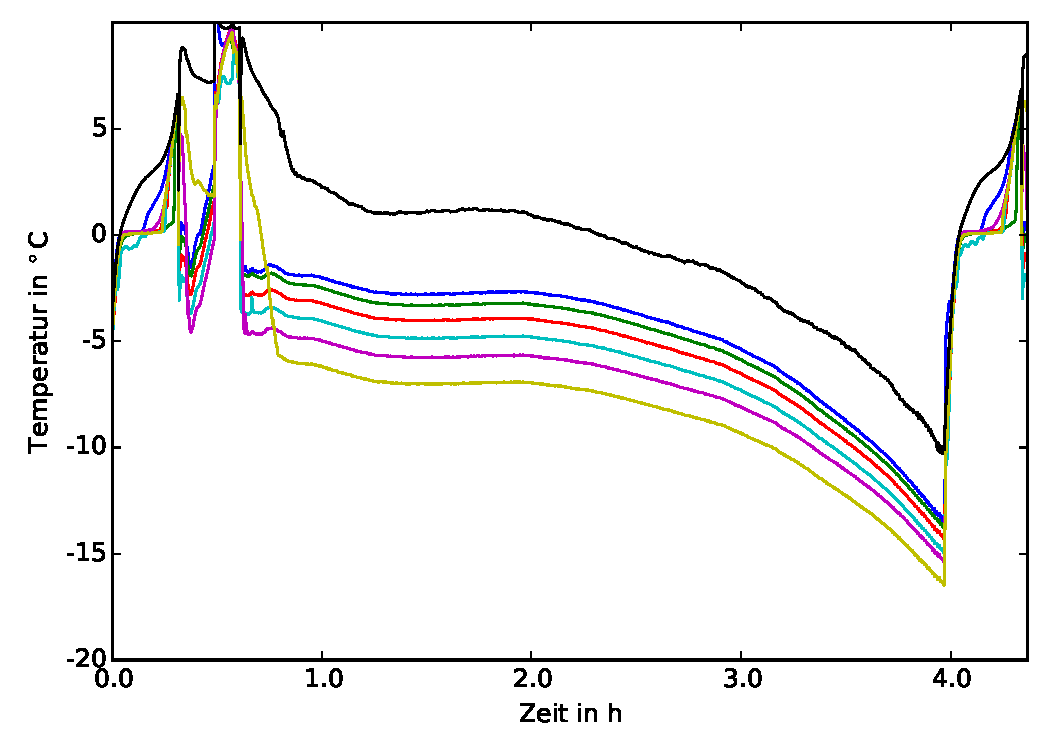
\includegraphics[scale=0.8]{Pictures/35/T_evap_C1_lastCycle.pdf}
\caption{Temperaturen im Verdampfer (K1) beim Betrieb mit 3MAF.}
\label{fig:deltaT35}
\end{figure}

\begin{figure}[h!]
\centering
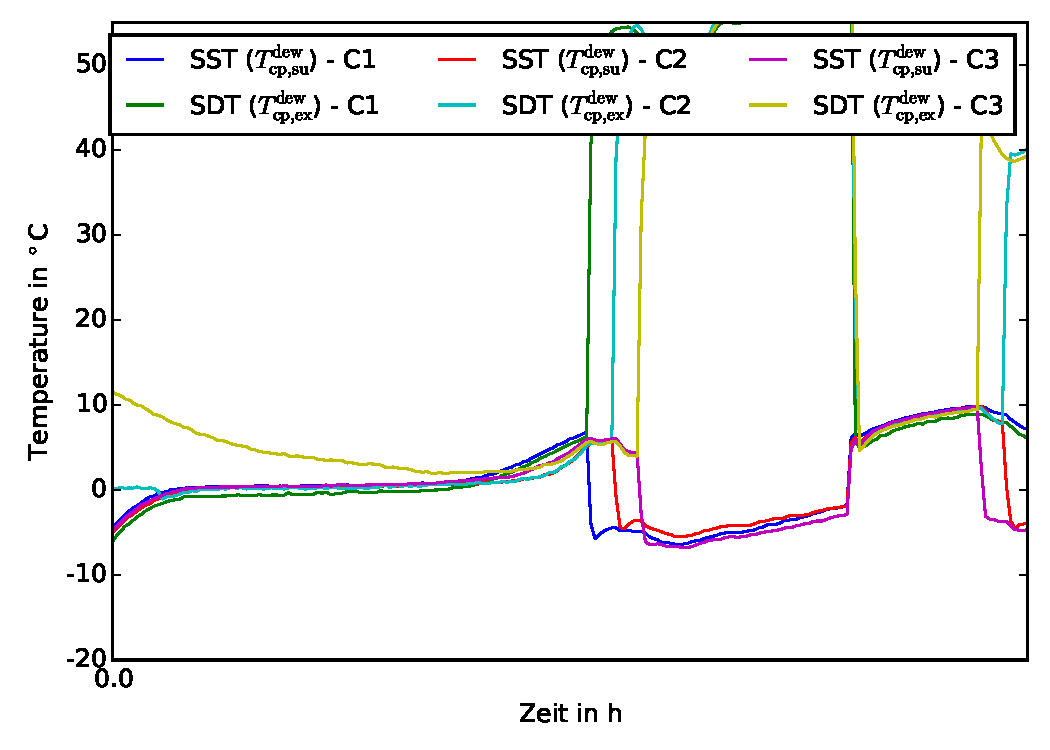
\includegraphics[scale=0.8]{Pictures/35/Tsats_lastCycle.pdf}
\caption{Sättigungstemperaturen (K1) beim Betrieb mit 3MAF.}
\label{fig:Tsats35}
\end{figure}

\begin{figure}[h!]
\centering
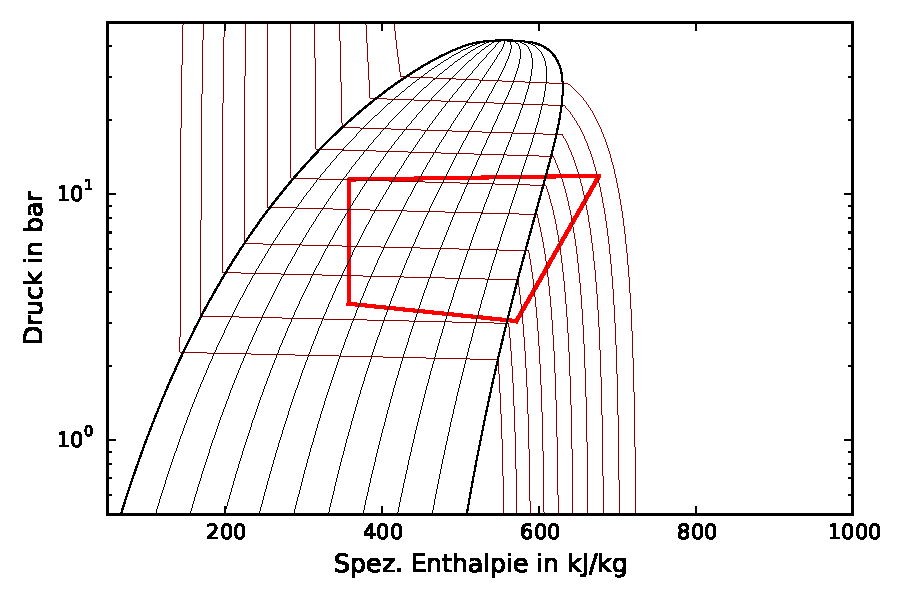
\includegraphics[scale=0.8]{Pictures/35/log_ph_lastCycle10perc_C1.pdf}
\caption{logp-h-Diagramm (K1) beim Betrieb mit 3MAF \unit{10}{\%} vor Ende des Zyklus.}
\label{fig:logph35}
\end{figure}

\begin{figure}[h!]
\centering
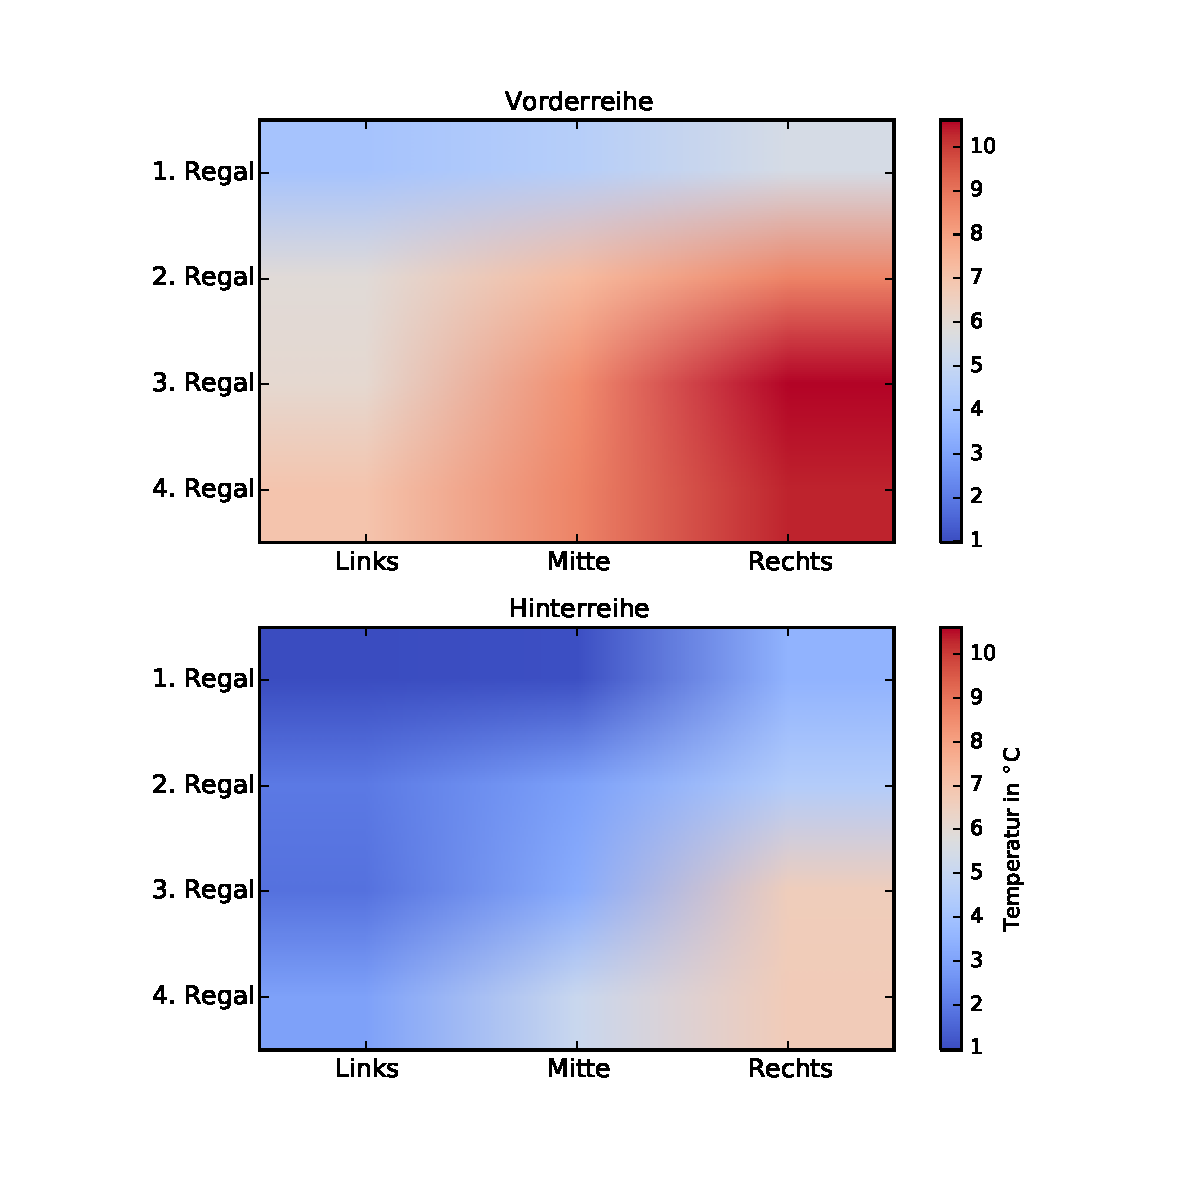
\includegraphics[scale=0.8]{Pictures/35/load_colormap_lastCycle10perc.pdf}
\caption{Produkttemperaturen in der vorderen und hinteren Regalreihe beim Betrieb mit 3MAF.}
\label{fig:prodtempmap35}
\end{figure}

\begin{figure}[h!]
\centering
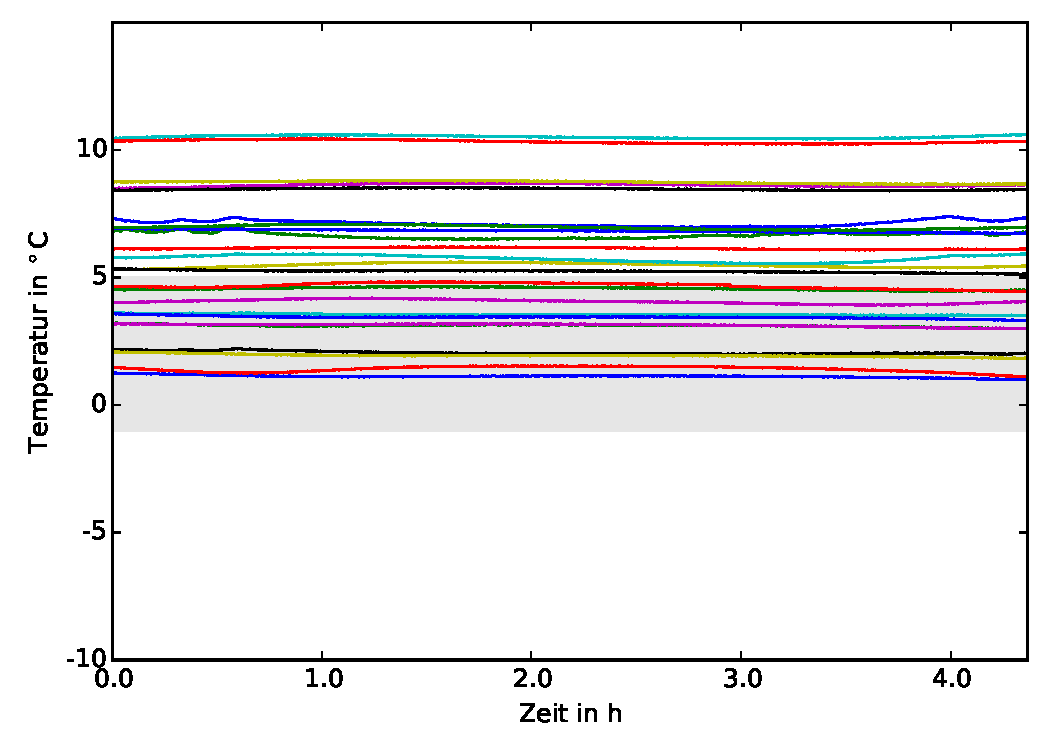
\includegraphics[scale=0.8]{Pictures/35/ProductTemperature.pdf}
\caption{Produkttemperaturen beim Betrieb mit 3MAF.}
\label{fig:prodtemp35}
\end{figure}



\section{Untersuchung 50}

\begin{figure}[h!]
\centering
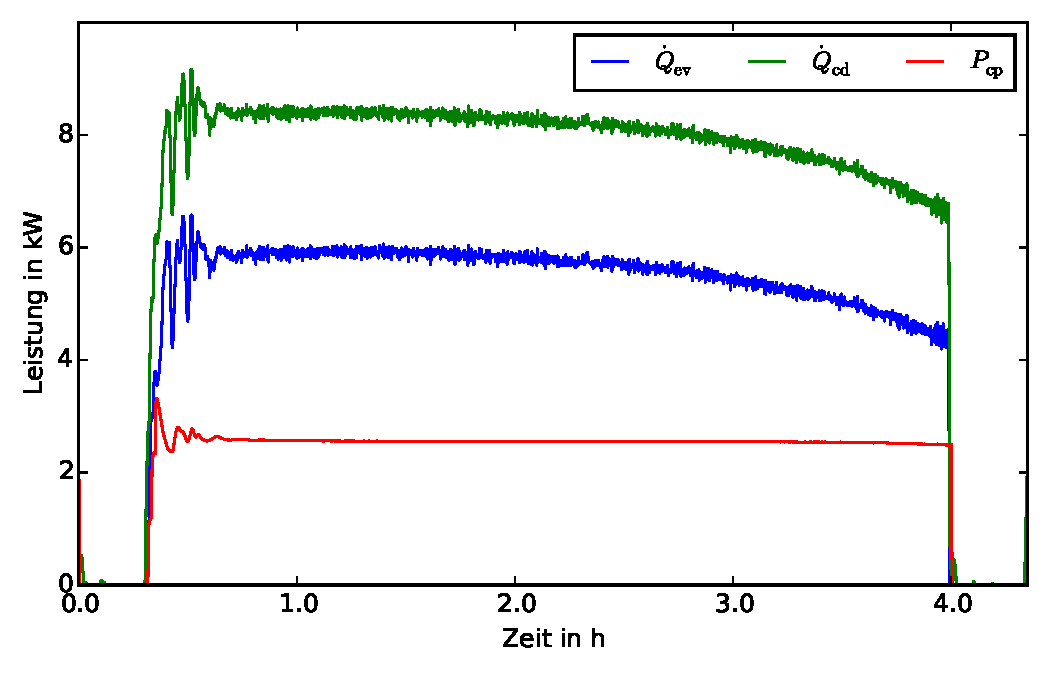
\includegraphics[scale=0.8]{Pictures/50/Qdots_lastCycle.pdf}
\caption{Leistungen beim Betrieb mit einem 4h Abtauintervall.}
\label{fig:Leistungen50}
\end{figure}

\begin{figure}[h!]
\centering
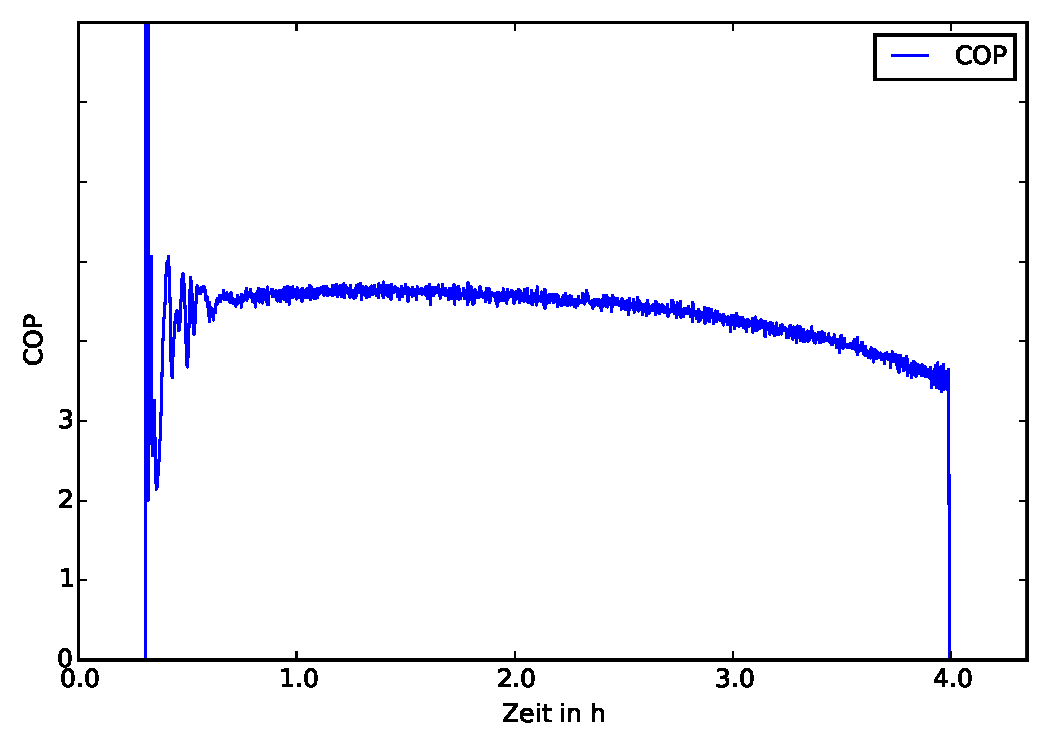
\includegraphics[scale=0.8]{Pictures/50/COP_lastCycle.pdf}
\caption{COP beim Betrieb mit einem 4h Abtauintervall.}
\label{fig:COP50}
\end{figure}

\begin{figure}[h!]
\centering
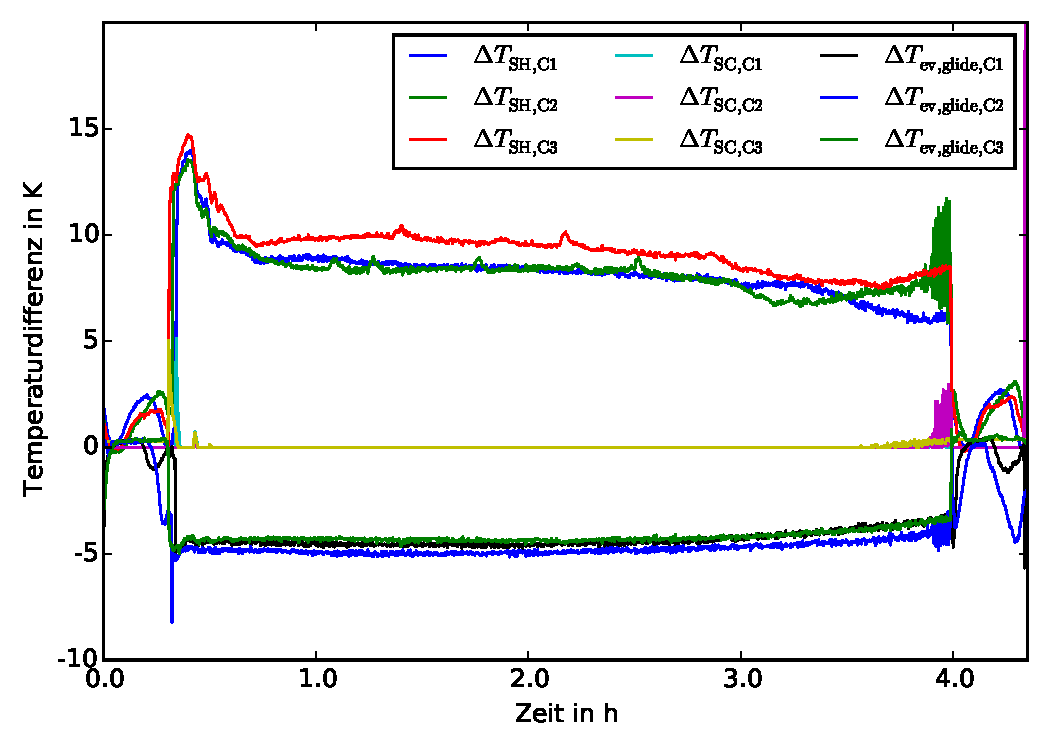
\includegraphics[scale=0.8]{Pictures/50/deltaTs_lastCycle.pdf}
\caption{Überhitzung und Unterkühlung (K1) beim Betrieb mit einem 4h Abtauintervall.}
\label{fig:deltaT50}
\end{figure}

\begin{figure}[h!]
\centering
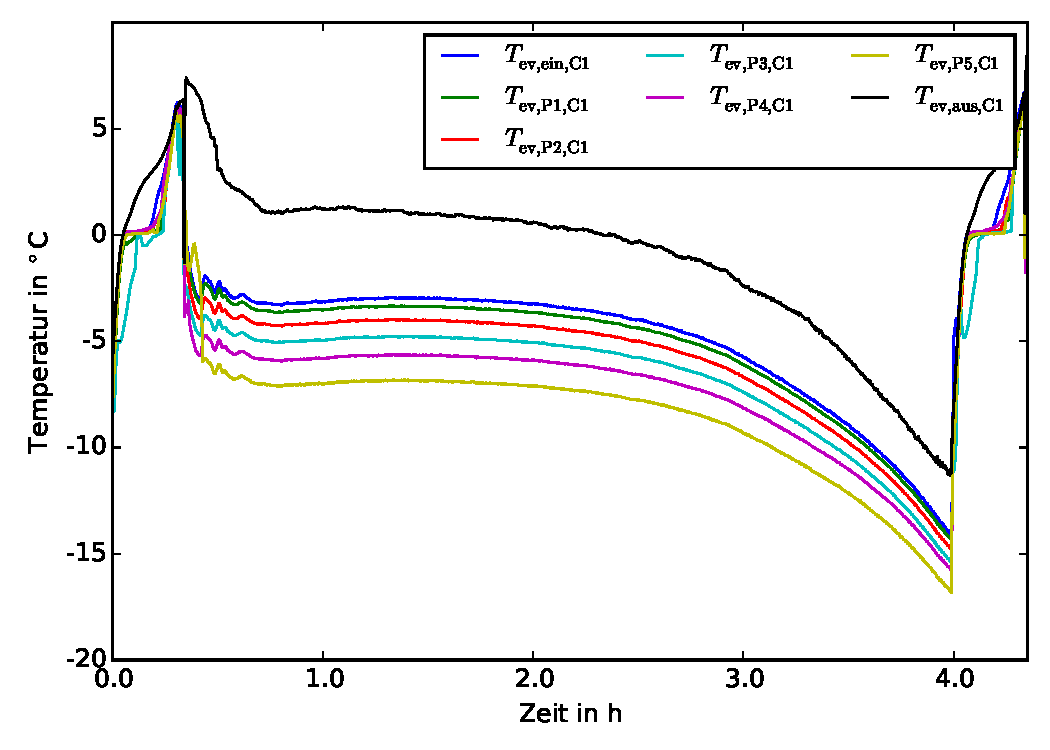
\includegraphics[scale=0.8]{Pictures/50/T_evap_C1_lastCycle.pdf}
\caption{Temperaturen im Verdampfer (K1) beim Betrieb mit einem 4h Abtauintervall.}
\label{fig:deltaT50}
\end{figure}

\begin{figure}[h!]
\centering
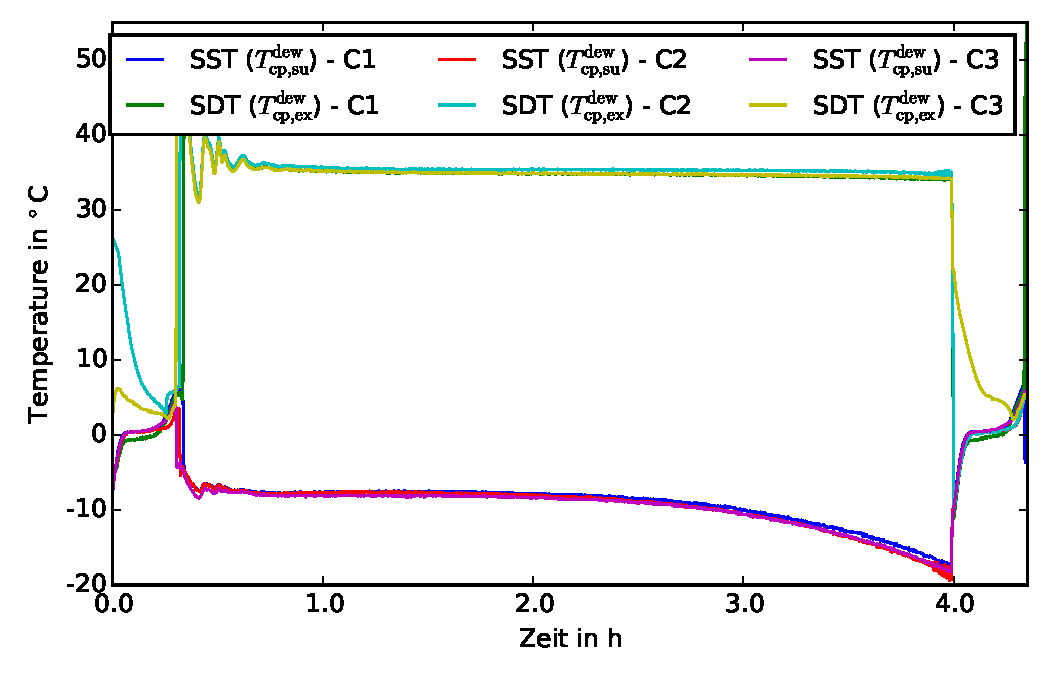
\includegraphics[scale=0.8]{Pictures/50/Tsats_lastCycle.pdf}
\caption{Sättigungstemperaturen (K1) beim Betrieb mit einem 4h Abtauintervall.}
\label{fig:Tsats50}
\end{figure}

\begin{figure}[h!]
\centering
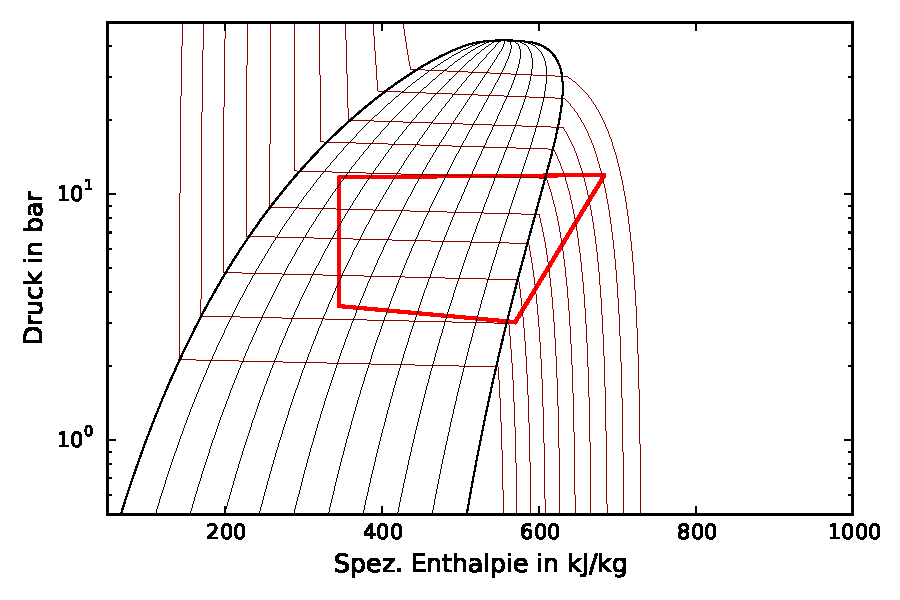
\includegraphics[scale=0.8]{Pictures/50/log_ph_lastCycle10perc_C1.pdf}
\caption{logp-h-Diagramm (K1) beim Betrieb mit einem 4h Abtauintervall \unit{10}{\%} vor Ende des Zyklus.}
\label{fig:logph50}
\end{figure}

\begin{figure}[h!]
\centering
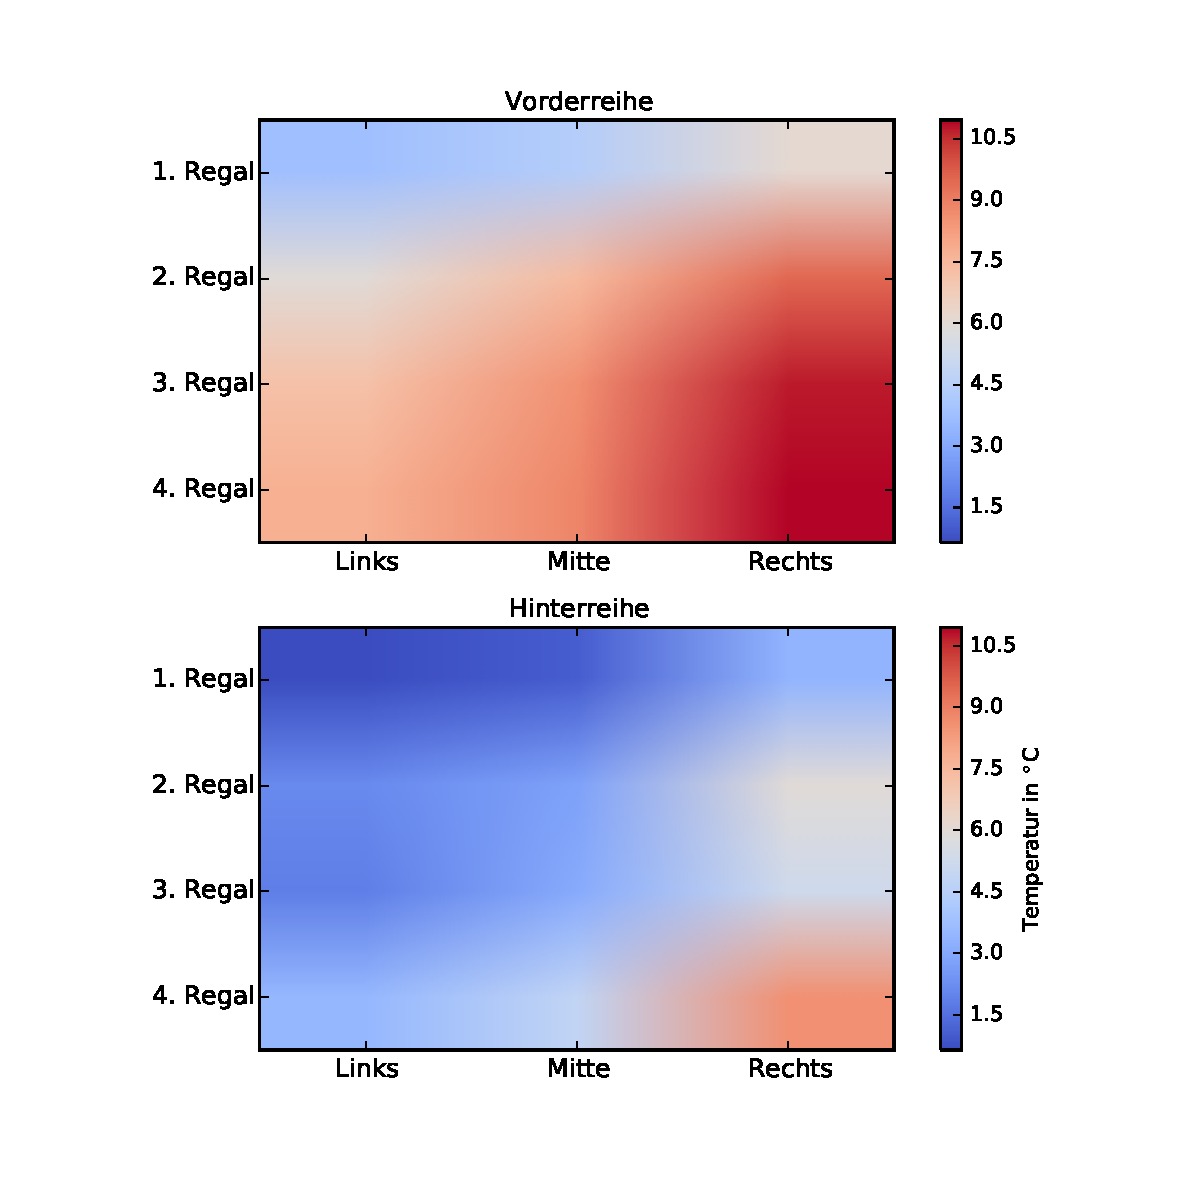
\includegraphics[scale=0.8]{Pictures/50/load_colormap_lastCycle10perc.pdf}
\caption{Produkttemperaturen in der vorderen und hinteren Regalreihe beim Betrieb mit einem 4h Abtauintervall.}
\label{fig:prodtempmap50}
\end{figure}

\begin{figure}[h!]
\centering
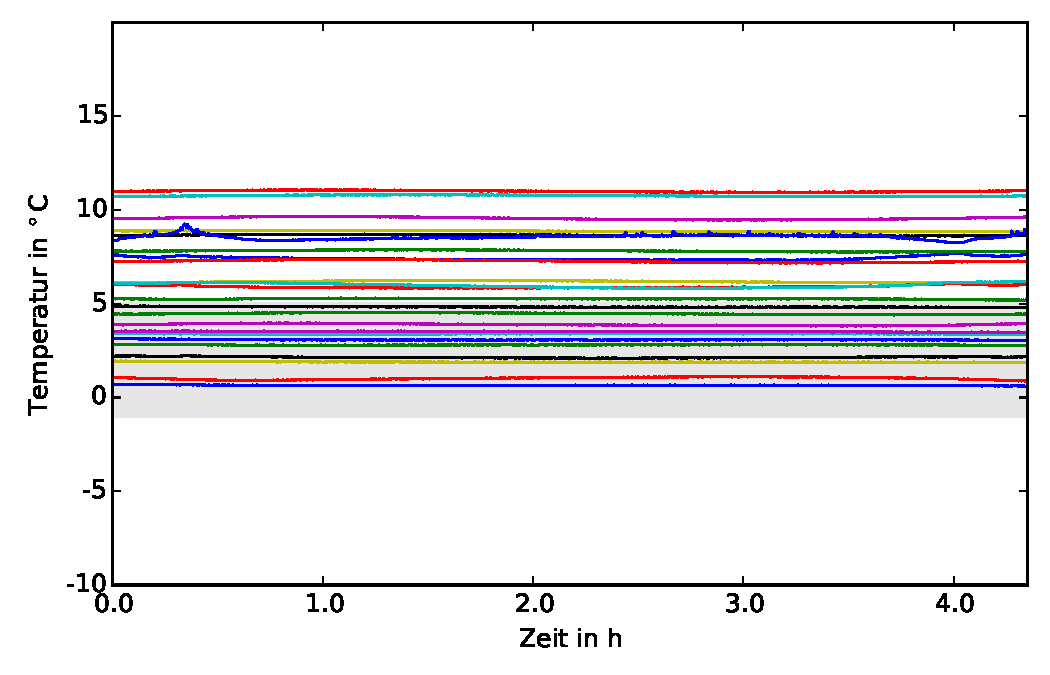
\includegraphics[scale=0.8]{Pictures/50/ProductTemperature.pdf}
\caption{Produkttemperaturen beim Betrieb mit einem 4h Abtauintervall.}
\label{fig:prodtemp50}
\end{figure}


\section{Betrieb mit 3h Abtauintervall}

\section{Betrieb mit ZB09KAU-TFD (Kupferwicklung)}

\section{Betrieb mit ZB09KAU-TFD (Aluminiumwicklung}

\section{Betrieb mit AHT Verdampfer}

\section{Betrieb mit LIDL Verdampfer V1 bei 0\% r.F.}

\section{Betrieb mit LIDL Verdampfer V1 bei 60\% r.F.}

\section{Betrieb mit LIDL Verdampfer V2 bei 0\% r.F.}

\section{Betrieb mit LIDL Verdampfer V2 bei 60\% r.F.}
